
\documentclass{article}
\usepackage[intlimits]{amsmath}
\usepackage{amssymb}
\usepackage{amsfonts,amstext,amsthm}
\usepackage{paralist}        % For {inparaenum} environment.
\usepackage{mathtools}       % For dcases.
\usepackage[normalem]{ulem}  % For strikethrough.
\usepackage[usenames,dvipsnames]{xcolor} % For named colors.
\usepackage{hyperref}        % For clickable refs.
\usepackage{subcaption}      % Allows to include subfigures, floats, etc.
%\usepackage{enumerate}
\usepackage{MnSymbol}

\usepackage[authoryear,sort]{natbib}
\hypersetup{
    unicode=false,          % non-Latin characters in Acrobat’s bookmarks
    pdftoolbar=true,        % show Acrobat’s toolbar?
    pdfmenubar=true,        % show Acrobat’s menu?
    pdffitwindow=false,     % window fit to page when opened
    pdfstartview={FitH},    % fits the width of the page to the window
    pdfnewwindow=true,      % links in new window
    colorlinks=true,        % false: boxed links; true: colored links
    linkcolor=red,          % color of internal links (change box color with linkbordercolor)
    citecolor=BrickRed,     % color of links to bibliography
    filecolor=BurntOrange,  % color of file links
    urlcolor=blue           % color of external links
} % \hypersetup
\renewcommand{\geq}{\geqslant}
\renewcommand{\leq}{\leqslant}

\usepackage[margin=2.5cm]{geometry}

\usepackage{graphicx}
\graphicspath{{./gfx/}}
\DeclareGraphicsExtensions{.eps}
\usepackage{epstopdf}
\usepackage{tikz}
\usetikzlibrary{arrows.meta}
\usetikzlibrary{calc}
\usetikzlibrary{patterns}

\renewcommand{\Pr}{\mathsf{P}}

%\usepackage[nott]{inconsolata} % for C++ code

% C++ styles.
%\newcommand{\cppfont}{\fontfamily{fi4}\selectfont}
%\newcommand{\cppkey}[1]{{\color{blue}#1}}
%\newcommand{\cppclass}[1]{{\color{mint}#1}}
%\newcommand{\cppparam}[1]{{\color{gray}#1}}

% Math
\newcommand{\slfrac}[2]{\left. #1 \middle/ #2 \right.}

% ~~ Theorems and such ~~
\newtheorem{theorem}{Theorem}
\newtheorem{lemma}{Lemma}
\newtheorem{corollary}{Corollary}
\newtheorem{proposition}{Proposition}
\theoremstyle{definition} %% or \theoremstyle{remark} will produce roman text
\newtheorem{definition}{Definition}
\newtheorem{remark}{Remark}
\newtheorem{assumption}{Assumption}
\newtheorem*{notation}{Notation}

\newtheorem{AUXalgorithm}{Algorithm}
\newenvironment{algorithm}[1]
  {\renewcommand\theAUXalgorithm{#1}\AUXalgorithm\begin{enumerate}\item[]}
  {\end{enumerate}\endAUXalgorithm}

% ~~ Math operators ~~
\DeclareMathOperator{\EV}{\mathbf{E}} % expected value
\DeclareMathOperator{\Var}{\mathbf{Var}} % variance
\DeclareMathOperator{\Cov}{\mathbf{Cov}} % covariance
\DeclareMathOperator{\Corr}{\mathbf{Corr}} % correlation
\DeclareMathOperator{\SD}{\mathbf{s.d.}} % standard deviation

% ~~ Distributions ~~
\DeclareMathOperator{\DBernoulli}{\mathrm{Bernoulli}} % Bernoulli distribution.
\DeclareMathOperator{\DNorm}{\mathcal{N}} % normal distribution
\DeclareMathOperator{\DLogNorm}{\ln \DNorm } % normal distribution
\DeclareMathOperator{\DExp}{\mathrm{Exp}} % exponential distribution
\DeclareMathOperator{\DPareto}{\mathrm{Pareto}} % exponential distribution
\DeclareMathOperator{\DBeta}{\mathrm{Be}} % exponential distribution
\DeclareMathOperator{\DUnif}{\mathrm{Uniform}} % exponential distribution
\newcommand{\scbeta}[1]{\DBeta_{\left(0, #1\right)}} % scaled beta distribution

% ~~ Misc ~~
\newcommand{\ignore}[1]{}
\newcommand{\nolabel}[1]{}
\newcommand{\cache}[1]{\fbox{$#1$}}
\newcommand{\ceil}[1]{\lceil{#1}\rceil}
\newcommand{\floor}[1]{\lfloor{#1}\rfloor}
\newcommand{\round}[1]{\lsem{#1}\rsem}
\newcommand{\Mode}{\theta}
\newcommand{\Reals}{\mathbb{R}}     % Real numbers.
\newcommand{\Integers}{\mathbb{Z}}  % Integer numbers.

% ~~ Set notation ~~
\newcommand{\set}[1]{\left\{ {#1} \right\}} % Set with automatically scaled parentheses: {...}.
\newcommand{\xset}[2][]{#1\{ {#2} #1\}}     % Set with custom scaled parentheses: {...}.
\newcommand{\cset}[3][\middle |]            % Set with condition: {... | ...}.
    {\left\{ {#2} \, #1 \, {#3} \right\}}

\begin{document}

\begin{notation}
    In this paper we will write $\floor{\cdot }$ for the floor function, and $\round{x} = \floor{x + 0.5}$ for the rounding function.
    The ``boxed'' \fbox{quantities} in the algorithms can be pre-computed to speed up calculations.
\end{notation}

\begin{assumption}
    In all of the algorithms we assume that all integers live in $\Integers / (M + 1)$, where $M$ is some positive integer.
\end{assumption}


\section{Bernoulli and Discrete Uniform distributions}

Before we proceed to more complicated algorithms, a couple of words on generating events with a prescribed probability $p$, $0 \leq p \leq 1$. Suppose $X \sim \DUnif \set{0, 1, \cdots , M}$. Note, that each value of $X$ occurs with probability $1 / (M + 1)$. Rounding $p$ to the nearest multiple of $1 / (M + 1)$ would be ideal, with the incurred error begin upper-bounded (sharply) by $0.5 / (M + 1)$:
\begin{center}
    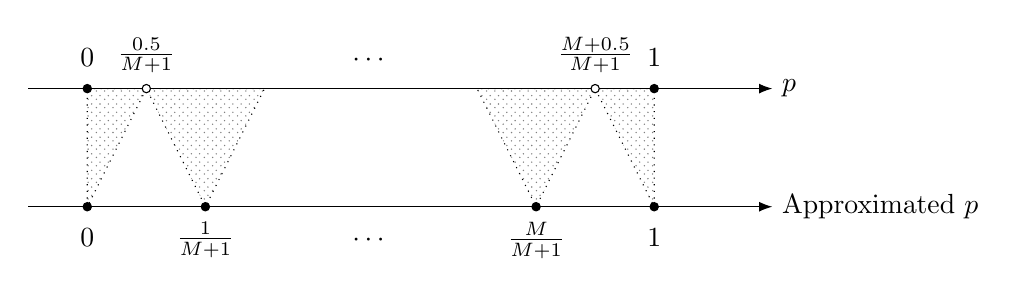
\begin{tikzpicture}[scale=1.5,
            axis/.style={->, >=Latex},
            tria/.style={pattern=north east lines, pattern color=gray,dotted},
            axpt/.style={color=black, fill=black},
            bxpt/.style={color=black},
            cxpt/.style={color=black, fill=white}]
        % ~~ Vertical alignment ~~
        \pgfmathsetmacro{\yTop}{1.5}
        \pgfmathsetmacro{\yBot}{0.5}
        % ~~ Horizontal alignment ~~
        \pgfmathsetmacro{\dx}{1.0}
        \pgfmathsetmacro{\xFirst}{1.5}
        \pgfmathsetmacro{\xLast}{6.3}
        % ~~ Axes ~~
        \draw[axis] (\xFirst - 0.5*\dx, \yTop) -- (\xLast + \dx, \yTop) node[right] {$\ensuremath{p}$};
        \draw[axis] (\xFirst - 0.5*\dx, \yBot) -- (\xLast + \dx, \yBot) node[right] {Approximated $\ensuremath{p}$};
        % ~~ Triangles (in-between vaues) ~~
        \draw[tria] (\xFirst, \yTop) -- (\xFirst + 0.5*\dx, \yTop) -- (\xFirst, \yBot) -- cycle;
        \draw[tria] (\xFirst + 0.5*\dx, \yTop) -- (\xFirst + 1.5*\dx, \yTop) -- (\xFirst + \dx, \yBot) -- cycle;
        \draw[tria] (\xLast - 0.5*\dx, \yTop) -- (\xLast - 1.5*\dx, \yTop) -- (\xLast - \dx, \yBot) -- cycle;
        \draw[tria] (\xLast, \yTop) -- (\xLast - 0.5*\dx, \yTop) -- (\xLast, \yBot) -- cycle;
        % ~~ Top labels ~~
        \draw[axpt] (\xFirst, \yTop)       circle (1.0pt) node[above, yshift=1.0ex] {$\ensuremath{0}$};
        \draw[cxpt] (\xFirst + 0.5*\dx, \yTop) circle (1.0pt) node[above, yshift=0.5ex] {$\ensuremath{\frac{0.5}{M + 1}}$};
        %\draw[axpt] (\xFirst + \dx, \yTop) circle (1.0pt) node[above, yshift=0.5ex] {$\ensuremath{\frac{1}{M + 1}}$};
        \draw (0.5*\xFirst + 0.5*\xLast, \yTop)           node[above, yshift=1.0ex] {$\ensuremath{\cdots }$};
        %\draw[axpt] (\xLast - \dx, \yTop)  circle (1.0pt) node[above, yshift=0.5ex] {$\ensuremath{\frac{M}{M + 1}}$};
        \draw[cxpt] (\xLast - 0.5*\dx, \yTop) circle (1.0pt) node[above, yshift=0.5ex] {$\ensuremath{\frac{M + 0.5}{M + 1}}$};
        \draw[axpt] (\xLast, \yTop)        circle (1.0pt) node[above, yshift=1.0ex] {$\ensuremath{1}$};
        % ~~ Bottom values ~~
        \draw[axpt] (\xFirst, \yBot)       circle (1.0pt) node[below, yshift=-1.0ex] {$\ensuremath{0}$};
        \draw[axpt] (\xFirst + \dx, \yBot) circle (1.0pt) node[below, yshift=-0.5ex] {$\ensuremath{\frac{1}{M + 1}}$};
        \draw[axpt] (0.5*\xFirst + 0.5*\xLast, \yBot)     node[below, yshift=-1.5ex] {$\ensuremath{\cdots }$};
        \draw[axpt] (\xLast - \dx, \yBot)  circle (1.0pt) node[below, yshift=-0.5ex] {$\ensuremath{\frac{M}{M + 1}}$};
        \draw[axpt] (\xLast, \yBot)        circle (1.0pt) node[below, yshift=-1.0ex] {$\ensuremath{1}$};
    \end{tikzpicture}
\end{center}
%
Unfortunately, this mapping yields $M + 2$ possible values, leading to technical complications, since we are restricted to $\Integers / (M + 1)$.
%
To address the issue, we round $p$ to the nearest multiple of $1 / M$ instead.
%
\begin{notation}
    For any $p$, $0 \leq p \leq 1$, we will write
    \[
        p ^\star = \begin{dcases}
            \, \round{M \, p} \quad & \text{if $0 \leq p \leq 0.5$}, \\
            \, M - \round{M (1 - p)} \quad & \text{if $0.5 < p \leq 1$}.
        \end{dcases}
    \]
\end{notation}
%
Events with probability $p$ may be approximated with either $\set{X < p^\star }$ or $\set{X \leq p^\star }$.
%
\begin{center}
    \renewcommand{\arraystretch}{1.4}
    \begin{tabular}{|c|c||c|c|}
        \hline
        Target probability                      & $p^\star $ & $\Pr (X < p^\star )$ & $\Pr (X \leq p^\star )$  \\ \hline\hline
        \hspace{2em} $0 \leq p < 0.5 / M$       & $0$        & $0$                  & $1 / (M + 1)$            \\ \hline
        $0.5 / M \leq p < 1.5 / M$              & $1$        & $1 / (M + 1)$        & $2 / (M + 1)$            \\ \hline
        \multicolumn{4}{c}{$\cdots $} \\ \hline
        $(M - 1.5) / M < p \leq (M - 0.5) / M$  & $M - 1$    & $(M - 1) / (M + 1)$  & $M / (M + 1)$            \\ \hline
        $(M - 0.5) / M < p \leq 1$ \hspace{5em} & $M$        & $M / (M + 1)$        & $1$                      \\ \hline
    \end{tabular}
\end{center}
%
It is not hard to see that this will lead to errors not exceeding $1.5 / M$.

\begin{algorithm}{(Bernoulli)}
    \item Let $p$, $0 \leq p \leq 1$, be the parameter of Bernoulli distribution. If $p = 1$, set $\cache{S} = 0$ and $\cache{H} = 1$.
    \item If $p < 1$, set $\cache{S} = 1$ and $\cache{H} = p^\star $.
    \item Generate $\hat{U} \sim \DUnif \set{0, 1, \cdots , M}$. If $\cache{S} \cdot \hat{U} < \cache{H}$ return \emph{true}, otherwise return \emph{false}.
\end{algorithm}
%
The algorithm above has $1 / M$ as an upper bound for the probabilities of generated events.
%
Now that we have a $\DBernoulli (p)$ generator, we will proceed to generation of $\DUnif \set{a, a + 1, \cdots , b}$, where $a \leq b$ are integers. Unlike the algorithm above, this generation can be done precisely with a rejection method. To this end, we will partition the set $\set{0, 1, \cdots , M}$ into blocks of size $(b - a + 1)$ with possibly one block of a smaller size. If the smaller block is selected---which happens with probability $((M + 1) \mod (b - a + 1)) / (M + 1)$---we start over.

\begin{algorithm}{(Discrete Uniform)}
    \item Let $a \leq b$ be the parameters of Uniform distribution, and set $\cache{N} = b - a$.
    \item If $\cache{N} = 0$, set $\cache{B} = M$.
    \item If $\cache{N} \neq 0$, set $\cache{B} = 1 + \floor{(M - \cache{N}) / (\cache{N} + 1)}$.
    \item \label{item:uniform:gen} Generate $\hat{U} \sim \DUnif \set{0, 1, \cdots , M}$, and set $K = \floor{\hat{U} / \,\cache{B}}$ to be the block index where $\hat{U}$ landed. Note that $K \mid \set{K \leq \cache{N}}$ is conditionally $\DUnif \set{0, 1, \cdots , \cache{N}}$.
    \item If $K \leq \cache{N}$, accept $a + K$.
    \item If $K > \cache{N}$, return to step \ref{item:uniform:gen}.
\end{algorithm}

\section{Discrete distributions with finite support}

\subsection{Overview}

In this section we will consider the so-called ``alias'' algorithm for generating random variates from discrete distributions with finite support, based off of a paper by \citet{Vose:91}.

\subsection{Formal Setup}

Suppose we are dealing with a random variable $X$ with a discrete distribution with finite support over $n \geq 1$ values:
\[
    \Pr (X = a_i) = p_i, \qquad 1 \leq i \leq n,
\]
with $p_1 + \cdots + p_n = 1$ and $p_i > 0$, $1 \leq i \leq n$. The algorithm is two-stage: at the first stage we select one of the elements with probability $(1/n)$; at the second stage we either take the chosen item, or its alias.
\begin{center}
    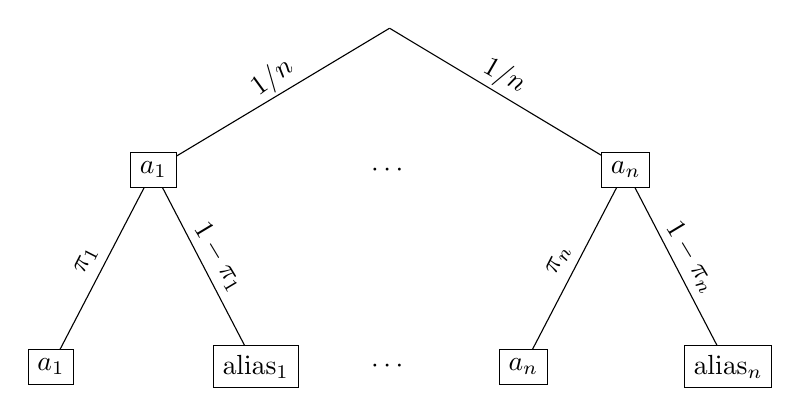
\begin{tikzpicture}
        \pgfmathsetmacro{\xSep}{3.0}
        \pgfmathsetmacro{\xxSep}{1.3}
        \pgfmathsetmacro{\ySep}{1.8}
        \pgfmathsetmacro{\yySep}{2.5}
        \coordinate (root) at (0, 0);
        % ~~ Top tier ~~
        \node[draw] (kk) at (-\xSep, -\ySep) {$\ensuremath{a_1}$};
        \draw (0, -\ySep) node {$\ensuremath{\cdots }$};
        \node[draw] (ll) at (\xSep, -\ySep) {$\ensuremath{a_n}$};
        % ~~ Bottom tier ~~
        \node[draw] (mm_kk) at (-\xSep-\xxSep, -\ySep-\yySep) {$\ensuremath{a_1}$};
        \node[draw] (nn_kk) at (-\xSep+\xxSep, -\ySep-\yySep) {$\ensuremath{\text{alias}_1}$};
        \draw (0, -\ySep-\yySep) node {$\ensuremath{\cdots }$};
        \node[draw] (mm_ll) at (\xSep-\xxSep, -\ySep-\yySep) {$\ensuremath{a_n}$};
        \node[draw] (nn_ll) at (\xSep+\xxSep, -\ySep-\yySep) {$\ensuremath{\text{alias}_n}$};
        % ~~ Edges ~~
        \draw (root) -- (kk) node[midway,rotate=36,yshift=1.5ex] {$\ensuremath{1/n}$};
        \draw (root) -- (ll) node[midway,rotate=-30,yshift=1.5ex] {$\ensuremath{1/n}$};
        \draw (kk) -- (mm_kk) node[midway,rotate=63,yshift=1.5ex] {$\ensuremath{\pi _1}$};
        \draw (kk) -- (nn_kk) node[midway,rotate=-59,yshift=1.5ex] {$\ensuremath{1 - \pi _1}$};
        \draw (ll) -- (mm_ll) node[midway,rotate=63,yshift=1.5ex] {$\ensuremath{\pi _n}$};
        \draw (ll) -- (nn_ll) node[midway,rotate=-59,yshift=1.5ex] {$\ensuremath{1 - \pi _n}$};
    \end{tikzpicture}
\end{center}
The idea behind setting up probabilities correctly is an iterative one, where at each step we eliminate one branch. More specifically, select $j$-th branch such that $p _j \leq 1/n$. Then setting $\pi _j = n \, p_j$ and ensuring that $j$-th element will not appear as an alias at future steps will take care of the left sub-branch. Choosing the $j$-th alias as any element, say $k$-th, with $p _k > 1/n$, and updating $p_k = p_k - (1 - \pi _j) / n$, will take care of the right sub-branch.

\subsection{Alias Algorithm}

\begin{algorithm}{(Continuous generators)}
    \item Create an array of conditional probabilities, $\cache{\pi _i }$, $1 \leq i \leq n$, and ``aliases'', $\cache{b_i} = \cache{a_i}$, $1 \leq i \leq n$.

    \item Categorize each probability as either ``small'' or ``large'':
        \[
            S = \cset{i}{p_i \leq 1/n}, \quad
            L = \cset{i}{p_i > 1/n}.
        \]

    \item While $S \neq \varnothing $ and $L \neq \varnothing $:
        \begin{enumerate}
            \item Take $j \in S$ (index of a small element) and $k \in L$ (index of a large element).
            \item Set $\cache{b_j} = \cache{a_k}$ (pair up the small element with the large element).
            \item Set $\cache{\pi _j} = n p_j \leq 1$ (record the cutoff value for the small element).
            \item Since this large element is now an ``alias'' for the small element, we will adjust the probability of it being selected in the future. Let $\delta _j = 1 / n - p_j \geq 0$ be the probability of element $k$ being selected in the $j$-th branch.
            \item Overwrite $p_k = p_k - \delta _j$, making sure that once we reach $k$-th branch, its chances of being selected will be smaller.
            \item If $p_k \leq 1 / n$, remove $k$ from $L$ and place it in $S$ (what used to be large is now small).
            \item Remove $j$ from $S$.
        \end{enumerate}

    \item For each $j \in S$ set $\cache{\pi _j} = 1$; for each $k \in L$ set $\cache{\pi _k} = 1$. This will mitigate some rounding errors.

    \item The steps above are the initialization stage and will have to be completed only once. The generation itself proceeds as follows:
        \begin{enumerate}
            \item Generate $K \sim \DUnif \set{1, \cdots , n}$.
            \item Generate $U \sim \DUnif [0, 1)$.
            \item If $U < \cache{\pi _K}$, accept $\cache{a_K}$.
            \item If $U \geq \cache{\pi _K}$, accept $\cache{b_K}$.
        \end{enumerate}
\end{algorithm}

\begin{algorithm}{(Discrete uniform integer generators)}
    \item Create an array of cutoff values, $\cache{\hat{\pi }_i }$, $1 \leq i \leq n$, and ``aliases'', $\cache{b_i} = \cache{a_i}$, $1 \leq i \leq n$.

    \item Categorize each probability as either ``small'' or ``large'':
        \[
            S = \cset{i}{n p_i \leq 1}, \quad
            L = \cset{i}{n p_i > 1}.
        \]

    \item While $S \neq \varnothing $ and $L \neq \varnothing $:
        \begin{enumerate}
            \item Take $j \in S$ (index of a small element) and $k \in L$ (index of a large element).
            \item Set $\cache{b_j} = \cache{a_k}$.
            \item Set $\cache{\hat{\pi }_j} = (n p_j)^\star \leq M$. If $n p_j = 1$, then set $\cache{b_j} = \cache{a_j}$.
            \item Set $\delta _j = 1 - n p_j \geq 0$.
            \item Overwrite $n p_k = n p_k - \delta _j$.
            \item If $n p_k \leq 1$, remove $k$ from $L$ and place it in $S$.
            \item Remove $j$ from $S$.
        \end{enumerate}

    \item For each $j \in S$ set $\cache{b_j} = \cache{a_j}$; for each $k \in L$ set $\cache{b_k} = \cache{a_k}$.

    \item The steps above are the initialization stage and will have to be completed only once. The generation itself proceeds as follows:
        \begin{enumerate}
            \item Generate $K \sim \DUnif \set{1, \cdots , n}$.
            \item Generate $\hat{U} \sim \DUnif \set{0, \cdots , M}$.
            \item If $\hat{U} < \cache{\hat{\pi }_K}$, accept $\cache{a_K}$.
            \item If $\hat{U} \geq \cache{\hat{\pi }_K}$, accept $\cache{b_K}$.
        \end{enumerate}
\end{algorithm}

\section{Unimodal absolutely continuous distributions}

\subsection{Overview}

The aim of this section is two-fold: first, to give an overview of the Ziggurat algorithm \citet{Marsaglia+Tsang} for unimodal absolutely continuous distributions; second, to provide one implementation if the algorithm. One of the beauties of the Ziggurat algorithm lies in the fact that while almost all the time it is a very efficient version of the classical rejection method, it allows to handle densities with infinite support---assuming it is known how to sample from the tail (in the normal case see, e.g., \citet{Marsaglia:64}).

\subsection{Formal Setup}

In what follows, let $f$ denote the density function; $\Mode $ denote the mode of the distribution (argument where $f$ achieves its maximum); and $T$ denote its survival function:
\[
    T(x) = \int _x ^{\infty} f(t) \,dt.
\]
We will start with the monotone decreasing density case; the monotone increasing case can be handled similarly.

The idea behind the Ziggurat algorithm is to cover the density function with $n \geq 2$ horizontal layers of the same area, where all the layers except for the bottom one are rectangular.
%
More formally, we start with a partition of the vertical interval
\[
    0 = f_0 < f_1 < \cdots < f_{n - 1} < f_{n} = f(\Mode ).
\]
For $1 \leq k \leq n - 1$ let
\begin{align*}
    a_k = \inf \big\{ x \,:\, f(x) > f_k \big\}, \quad
    b_k = \sup \big\{ x \,:\, f(x) > f_k \big\};
\end{align*}
put $a_n = b_n = \Mode $, and define the layers by
\begin{align*}
    \begin{dcases}
        L_0 = \big\{ (x, y) \,:\, 0 \leq y \leq \min \{f_1, f(x)\} \big\}, \\
        L_k = [a_k, b_k] \times [f_k, f_{k + 1}], \quad 1 \leq k \leq n - 1.
    \end{dcases}
\end{align*}
This layering is illustrated in Figure~\ref{fig:ziggurat:3_layers}.

\begin{figure}[!ht]
    \centering
    \newcommand{\xfactor}{4.5}
    \newcommand{\yfactor}{8.5}
    \newcommand{\plotfun}[1]{\yfactor * #1 * exp(-#1 * #1)}
    \newcommand{\plotcoord}[2]{(\xfactor*#1,{\plotfun{#2}})}
    \newcommand{\plotMode}{0.7071}
    \newcommand{\plotZero}{0}
    \newcommand{\plotAone}{0.1536} % unscaled f_1 = 0.15
    \newcommand{\plotAtwo}{0.2687} % unscaled f_2 = 0.25
    \newcommand{\plotBtwo}{1.2770} % unscaled f_2 = 0.25
    \newcommand{\plotBone}{1.5223} % unscaled f_1 = 0.15
    \newcommand{\plotXfrom}{0.0}
    \newcommand{\plotXto}{1.8}
    \begin{tikzpicture}[scale=1.0, >=Latex,
            every node/.style={anchor=base},
            help lines/.style={dashed, thick},
            axis/.style={<->},
            important line/.style={thick},
            connection/.style={thick, dotted}]
        % ~~ Rectangular layers ~~
        \draw[pattern=north west lines, pattern color=gray] \plotcoord{\plotAtwo}{\plotMode} rectangle \plotcoord{\plotBtwo}{\plotBtwo}
            node[above right, yshift=4ex] {$\ensuremath{L_2}$};
        \draw[pattern=north east lines, pattern color=gray] \plotcoord{\plotAone}{\plotBtwo} rectangle \plotcoord{\plotBone}{\plotBone}
            node[above right, yshift=2ex] {$\ensuremath{L_1}$};
        % ~~ Bottom layer ~~
        \fill[pattern=dots, pattern color=gray] plot[domain=\plotXfrom:\plotXto] (\xfactor*\x,{min(\plotfun{\plotBone},\plotfun{\x})})--(\xfactor*\plotXto,0)--(\xfactor*\plotXfrom,0)--cycle;
        \draw \plotcoord{\plotXto}{\plotXto} node[above right, yshift=-2ex] {$\ensuremath{L_0}$};
        % ~~ Density ~~
        \draw[important line] plot[smooth,domain=\plotXfrom:\plotXto] (\xfactor*\x,{\plotfun{\x}}) node[right] {};

        \draw[connection]
            \plotcoord{\plotAone}{\plotAone}--(\xfactor*\plotAone,0.0)
            \plotcoord{\plotAtwo}{\plotAtwo}--(\xfactor*\plotAtwo,0.0)
            \plotcoord{\plotMode}{\plotMode}--(\xfactor*\plotMode,0.0)
            \plotcoord{\plotBone}{\plotBone}--(\xfactor*\plotBone,0.0)
            \plotcoord{\plotBtwo}{\plotBtwo}--(\xfactor*\plotBtwo,0.0);

        \draw (\xfactor*\plotAone,-0.4) node {$\ensuremath{a_1}$};
        \draw (\xfactor*\plotAtwo,-0.4) node {$\ensuremath{a_2}$};
        \draw (\xfactor*\plotMode,-0.4) node {$\ensuremath{a_3 = \Mode = b_3}$};
        \draw (\xfactor*\plotBtwo,-0.4) node {$\ensuremath{b_2}$};
        \draw (\xfactor*\plotBone,-0.4) node {$\ensuremath{b_1}$};

        \draw[connection] \plotcoord{\plotAtwo}{\plotMode}--\plotcoord{\plotZero}{\plotMode} node[left] {$\ensuremath{f_3 = f(\Mode )}$};
        \draw[connection] \plotcoord{\plotAone}{\plotBtwo}--\plotcoord{\plotZero}{\plotBtwo} node[left] {$\ensuremath{f_2}$};
        \draw[connection] \plotcoord{\plotAone}{\plotBone}--\plotcoord{\plotZero}{\plotBone} node[left] {$\ensuremath{f_1}$};
        \draw[connection] (\xfactor*\plotZero,0.0) node[left] {$\ensuremath{f_0 = 0}$};

        % ~~ Axes ~~
        \draw[->] (\xfactor*\plotZero,-0.2)--(\xfactor*\plotZero,4.3); % Vertical axis.
        \draw[->] (-0.1+\xfactor*\plotXfrom,0.0)--(0.4+\xfactor*\plotXto,0.0); % Horizontal axis.
    \end{tikzpicture}
    \caption{Unimodal Ziggurat algorithm with $3$ layers.}
    \label{fig:ziggurat:3_layers}
\end{figure}
%
We want to choose $f_1, \cdots , f_{n - 1}$ in such a way as to make sure that the area of each layer is the same:
\[
    |L_0| = |L_1| = \cdots = |L_{n - 1}| = V.
\]
Thus, one arrives at a (non-linear) system of $n$ equations with $n$ unknowns:
\begin{align} \label{eq:zigg_system}
    \begin{dcases}
        V = (1 - T(a_1)) + (b_1 - a_1) \, f_1 + T(b_1) \\
        V = (b_k - a_k) \, \big( f_{k + 1} - f_k \big), \quad 1 \leq k \leq n - 1.
    \end{dcases}
\end{align}

\begin{proposition}
    System \eqref{eq:zigg_system} has a unique solution.
\end{proposition}

Having set up the basics, let us review the principles of the Ziggurat algorithm.
\begin{itemize}
    \item The first step is to select one layer (uniformly) at random.
    \item The second step is to generate a (uniform) random point inside the selected layer. If the point happens to be under the graph of the density function, we accept it. Otherwise, we start over from the first step.
\end{itemize}

To facilitate these steps, note that every layer has a rectangular subset that lies entirely under the density curve. Specifically, all
\[
    B_k = [a_{k + 1} , b_{k + 1}] \times [f_k, f_{k + 1}] \subseteq L_k, \quad 0 \leq k \leq n - 1,
\]
lie under the graph of $f$ (for the top layer the box $B_{n - 1}$ is trivial).
In light of this, the second step of the algorithm becomes substantially simpler if the point sampled from layer $L_k$ falls inside $B_k$. The probability of this happening, which we will refer to as the \emph{simple coverage probability}, is
\[
    p_k = \frac{|B_k|}{|L_k|}.
\]
It is convenient to write these probabilities in terms of the widths of the layers (the term ``width'' is accurate for all layers but the bottom one, in which case we interpret it as the width of a rectangle of the same height and area). Let
\[
    a_0 = a_1 - (1 - T(a_1)) / f_1
    \quad \text{and} \quad
    b_0 = b_1 + T(b_1) / f_1,
\]
and set
\begin{align} \label{eq:layer_width}
    \begin{dcases}
        %w_0 = V / f_1, \\
        w_k = b_k - a_k, \quad 0 \leq k \leq n - 1, \\
        w_n = 0.
    \end{dcases}
\end{align}
Then the simple coverage probabilities become
\begin{align} \label{eq:simple_coverage_probability}
    p_k &= \frac{w_{k + 1}}{w_{k}} \quad \text{for $0 \leq k \leq n - 1$}.
\end{align}
%
Furthermore, let $\alpha _k$ and $\beta _k$, $0 \leq k \leq n - 1$, denote the probabilities of landing to the left and right of $B_k$, respectively. Then
\begin{align} \label{eq:fallout_probability}
    \begin{dcases}
        \alpha _k = (a_{k + 1} - a_{k}) / w_k, \\
        \beta _k = (b_{k} - b_{k + 1}) / w_k,
    \end{dcases}
    \quad \text{for $0 \leq k \leq n - 1$}.
\end{align}
Note, that in the case of monotone densities, either all $\alpha _k = 0$ or all $\beta _k = 0$, $0 \leq k \leq n - 1$.
%
It is not difficult to see that
\begin{align*}
    \Pr \big(\text{simple coverage}\big) &= \frac{1}{n} \sum _{k = 0} ^{n - 1} \Pr \big(\text{simple coverage} \mid \text{layer $k$}\big)
        = \frac{p_0 + \cdots + p_{n - 1}}{n}, \\
    \Pr \big(\text{rejection}\big) &= \frac{1}{n} \sum _{k = 0} ^{n - 1} \Pr \big(\text{rejection} \mid \text{layer $k$}\big)
        = 1 - \frac{1}{n V}.
\end{align*}


\subsection{Ziggurat Algorithm}

The algorithm of \citet{Marsaglia+Tsang} and \citet{Doornik:05} for $n \geq 2$ layers is summarized below.

\begin{algorithm}{(Continuous generators)}
    \item \label{item:alg_cont:choose_box} Generate $K \sim \DUnif \{ 0, 1, \cdots , n - 1 \}$, the zero-based layer index.

    \item \nolabel{item:alg_cont:horizontal} Generate $U \sim \DUnif [0, 1)$, the relative ``horizontal position'' inside $L_K$.

    \item \nolabel{item:alg_cont:bottom_layer} If $K = 0$:
        \begin{enumerate}
            \item If $U < \cache{\alpha _0}$, accept a variate from the left tail.
            \item If $U \geq \cache{1 - \beta _0}$, accept a variate from the right tail.
            \item If $\cache{\alpha _0} \leq U < \cache{1 - \beta _0}$, accept $\cache{a_0} + U \cdot \cache{w_0}$, since the random point landed inside $B_0$.
        \end{enumerate}

    \item \nolabel{item:alg_cont:other_layers} If $K \neq 0$:
        \begin{enumerate}
            \item Let $X = \cache{a_K} + U \cdot \cache{w_K}$ be the abscissa of the random point inside $L_K$.
            \item If $\cache{\alpha _K} \leq U < \cache{1 - \beta _K}$, accept $X$, since the point landed inside $B_K$.
            \item Generate $W \sim \DUnif [0, 1)$, the relative vertical position inside $L_K$.
            \item If $\cache{f_K} + W \cdot \cache{(f_{K + 1} - f_{K})} < f(X)$, accept $X$, since the point landed under the graph of $f$.
            \item Return to step \ref{item:alg_cont:choose_box}.
        \end{enumerate}
\end{algorithm}

In practice one usually has to deal with discrete uniform integer generators. For simplicity of presentation, we will assume that the possible values are $\{ 0, 1, \cdots , M \}$; typically, $M$ would be a Mersenne number.
The previous algorithm can be adjusted to take advantage of integer arithmetic in the following way:
\begin{algorithm}{(Discrete uniform integer generators)}
    \item \label{item:alg_disc:choose_box} Generate $K \sim \DUnif \{ 0, 1, \cdots , n - 1 \}$, the zero-based layer index.

    \item \nolabel{item:alg_disc:horizontal} Generate $\hat{U} \sim \DUnif \{ 0, 1, \cdots , M \}$, the up-scaled relative ``horizontal position'' inside $L_K$.

    \item \nolabel{item:alg_disc:bottom_layer} If $K = 0$:
        \begin{enumerate}
            \item If $\hat{U} < \cache{\round{(M^\star + 1) \alpha _0}}$, accept a variate from the left tail.
            \item If $\hat{U} > \cache{\round{(M^\star + 1) (1 - \beta _0)}}$, accept a variate from the right tail.
            \item If $\cache{\round{(M^\star + 1) \alpha _0}} \leq \hat{U} \leq \cache{\round{(M^\star + 1) (1 - \beta _0)}}$, accept $\cache{a_0} + \hat{U} \cdot \cache{w_0  / (M + 1)}$, since the random point landed inside $B_0$.
        \end{enumerate}

    \item \nolabel{item:alg_disc:other_layers} If $K \neq 0$:
        \begin{enumerate}
            \item Let $X = \cache{a_K} + \hat{U} \cdot \cache{w_K / (M + 1)}$ be the abscissa of the random point inside $L_K$.
            \item If $\cache{\round{(M^\star + 1) \alpha _K}} < \hat{U} < \cache{\round{(M^\star + 1) (1 - \beta _K)}}$, accept $X$, since the point landed inside $B_K$.
            \item Generate $\hat{W} \sim \DUnif \{0, 1, \cdots , M \}$, the up-scaled relative vertical position inside $L_K$.
            \item If $\cache{f_K} + \hat{W} \cdot \cache{(f_{K + 1} - f_{K}) / (M + 1)} < f(X)$, accept $X$, since the point landed under the graph of $f$.
            \item Return to step \ref{item:alg_disc:choose_box}.
        \end{enumerate}
\end{algorithm}
%
Note, that if we know in advance that $\alpha _0 = \cdots = \alpha _{n - 1} = 0$ or $\beta _0 = \cdots = \beta _{n - 1} = 0$, certain steps in the algorithm can be simplified (or skipped entirely).

\begin{remark}
    In most cases, we think it is reasonable to make the following assumptions.
    \begin{itemize}
        \item If $\alpha _j = 0$ for some $j$, then all $\alpha _k = 0$, $0 \leq k \leq n - 1$.
        \item If $\beta _j = 0$ for some $j$, then all $\beta _k = 0$, $0 \leq k \leq n - 1$.
    \end{itemize}
\end{remark}

\begin{remark}
    Also note, that only $\ceil{\log _2 (n)}$ bits are necessary to generate $K$; the remaining bits may be used, e.g., to implement vectorized Ziggurat versions, or store the random index for repeated iterations.
\end{remark}

\bibliographystyle{plainnat}
\bibliography{samplers}


\end{document}
